%QQQ Below: "10pt" prints in 10-point. "12pt" prints in larger 12-point.
\documentclass[12pt,letterpaper]{article}
\usepackage{amsthm,amssymb,amsmath}
\usepackage[pdftex]{hyperref}
\usepackage{tikz}
%QQQ To print single-spaced, comment out the line below (precede it with a "%").
%QQQ To print double-spaced, remove the "%" at the beginning of the line.
%\renewcommand{\baselinestretch}{2}

% TIKZ

\pgfdeclarelayer{bg}    % declare background layer
\pgfsetlayers{bg,main}  % set the order of the layers

\tikzset{every label/.append style={fill=white}}
\tikzset{
    every node/.style={circle, fill, draw, minimum size=1mm, scale=.6,
    	font=\LARGE}
}

% MARGINS

\setlength{\textwidth}{6.3in}
\setlength{\textheight}{8.7in}
\setlength{\topmargin}{0pt}
\setlength{\headsep}{0pt}
\setlength{\headheight}{0pt}
\setlength{\oddsidemargin}{0pt}
\setlength{\evensidemargin}{0pt}

% SET UP SECTION NUMBERING

\setcounter{secnumdepth}{1}
% Number sections, but not subsections

% BREAK THEOREM STYLE

\newtheoremstyle{break}% name
  {}%         Space above, empty = `usual value'
  {}%         Space below
  {}% Body font
  {}%         Indent amount (empty = no indent, \parindent = para indent)
  {\bfseries}% Thm head font
  {.}%        Punctuation after thm head
  {\newline}% Space after thm head: \newline = linebreak
  {}%         Thm head spec

% DEFINE THEOREM-LIKE STRUCTURES

\theoremstyle{plain}
\newtheorem{lemma}{Lemma}[section]           % L:
%\newtheorem{lemma}{Lemma}                    % L:
\newtheorem{proposition}[lemma]{Proposition} % P:
\newtheorem{theorem}[lemma]{Theorem}         % T:
\newtheorem{corollary}[lemma]{Corollary}     % C:
\newtheorem{conjecture}[lemma]{Conjecture}   % J:
\newtheorem{question}[lemma]{Question}       % Q:
\newtheorem{problem}[lemma]{Problem}         % B:

\newtheorem{observation}[lemma]{Observation} % O:
\newtheorem{remark}[lemma]{Remark}           % R:

\theoremstyle{definition}
\newtheorem{definition}[lemma]{Definition}   % D:
\newtheorem{example}[lemma]{Example}         % E:

\theoremstyle{break}
\newtheorem{algorithm}[lemma]{Algorithm}     % A:
\newtheorem{implementation}[lemma]{Implementation}     % A:

% Also: Section = S:, Figure = Fig:, Item = It:, Equation = Eq:

% CHANGE APPEARANCE OF ENUMERATED LISTS

\renewcommand{\labelenumi}{(\roman{enumi})} % Labels (i), (ii), etc.

% CHANGE QED-RELATED COMMANDS

\renewcommand{\qed}{}
\newcommand{\ggcqedsymbol}{$\square$}
\newcommand{\ggcqed}{\hbox{}\nobreak\hbox{\quad\ggcqedsymbol}}
\newcommand{\ggcendpf}{\ggcqed}
%\newcommand{\ggcnopf}{}
\newcommand{\ggcnopf}{\ggcqed}
%\newcommand{\ggcendexample}{}
\newcommand{\ggcendexample}{\ggcqed}

% SET STYLE FOR DEFINED TERMS

\newcommand{\defterm}[1]{\emph{#1}} % Defined term
\newcommand{\abstdefterm}[1]{#1} % Defined term in abstract
\newcommand{\localdefterm}[1]{\emph{#1}} % Defined term used only nearby

% RUN-IN HEADINGS

\newcommand{\runinhead}[1]{\vskip0.1in\noindent\textbf{#1}} % Run-in heading
% This should be used at the start of a paragraph,
%  with no space between it and the first word of the paragraph.

% DEFINITIONS SPECIFIC TO THIS DOCUMENT

% (NONE)

\date{June 1, 2017}

\title{Path-Coloring Algorithms for Plane Graphs}

\author{Aven Bross\\
\small Department of Computer Science\\
\small University of Alaska\\
\small Fairbanks, AK 99775-6670\\
\small\texttt{dabross@alaska.edu} \and
Glenn G.~Chappell\\
\small Department of Computer Science\\
\small University of Alaska\\
\small Fairbanks, AK 99775-6670\\
\small\texttt{chappellg{@}member.ams.org} \and
Chris Hartman\\
\small Department of Computer Science\\
\small University of Alaska\\
\small Fairbanks, AK 99775-6670\\
\small\texttt{cmhartman{@}alaska.edu}}

\begin{document}

\maketitle
\centerline{\small \textit{2010 Mathematics Subject Classification.}
 Primary 05C38; Secondary 05C10, 05C15.}
\centerline{\small \textit{Key words and phrases.}
 Path coloring, list coloring, algorithm.}

\begin{abstract}
A \abstdefterm{path coloring} of a graph $G$ is a vertex coloring
of $G$ such that each color class induces a disjoint union of paths.
We present two efficient algorithms
to construct a path coloring of a plane graph.

The first algorithm, based on a proof of Poh, %\cite{Poh1990}
is given a plane graph;
it produces a path coloring of the given graph
using three colors.

The second algorithm,
based on similar proofs
by Hartman % \cite{Har1997}
and \v{S}krekovski, %\cite{Skr1999}
performs a list-coloring generalization of the above.
The algorithm is given a plane graph and an assignment of lists of
three colors to each vertex;
it produces a path coloring of the given graph
in which each vertex receives a color from its list.

Implementations of both algorithms are available.
\end{abstract}


\section{Introduction}

All graphs will be finite, simple, and undirected.
See West~\cite{Wes2000} for graph theoretic terms.

A \defterm{path coloring} of a graph $G$ is a vertex coloring
(not necessarily proper) of $G$ such that each color class induces
a disjoint union of paths.
A graph $G$ is \defterm{path $k$-colorable} if $G$
admits a path coloring using $k$ colors.

Broere \& Mynhardt conjectured~\cite[Conj.~16]{BrMy1985}
that every planar graph is path $3$-colorable.
This was proven independently by Poh~\cite[Thm.~2]{Poh1990}
and by Goddard~\cite[Thm.~1]{God1991}.

\begin{theorem}[Poh 1990, Goddard 1991] \label{T:planar3c}
If $G$ is a planar graph,
then $G$ is path $3$-colorable.\ggcnopf\end{theorem}

It is easily shown that the ``$3$'' in Theorem~\ref{T:planar3c}
is best possible.
In particular, Chartrand \& Kronk~\cite[Section~3]{ChKr1969}
gave an example of a planar graph whose vertex set cannot be partitioned
into two subsets, each inducing a forest.

Hartman~\cite[Thm.~4.1]{Har1997}
proved a list-coloring generalization of Theorem~\ref{T:planar3c}
(see also Chappell \& Hartman~\cite[Thm.~2.1]{ChHa2017prep}).
A graph $G$ is \defterm{path $k$-choosable} if,
whenever each vertex of $G$ is assigned a list of $k$ colors,
there exists a path coloring of $G$ in which each vertex receives
a color from its list.

\begin{theorem}[Hartman 1997] \label{T:planar3}
If $G$ is a planar graph,
then $G$ is path $3$-choosable.\ggcnopf\end{theorem}

Essentially the same technique was used by
\v{S}krekovski~\cite[Thm.~2.2b]{Skr1999}
to prove a result slightly weaker than Theorem~\ref{T:planar3}.


\medskip

We discuss two efficient path-coloring algorithms
based on proofs of the above theorems.
We distinguish between a \defterm{planar} graph---one that
can be drawn in the plane without crossing edges---and
a \defterm{plane} graph---a graph with a given embedding
in the plane.

In Section~2 we outline our graph representations
and the basis for our computations of time complexity.

Section~3 covers an algorithm
based on Poh's proof of Theorem~\ref{T:planar3c}.
The algorithm is given a plane graph;
it produces a path coloring of the given graph
using three colors.

Section~4 covers an algorithm
based Hartman's proof of Theorem~\ref{T:planar3},
along with the proof of \v{S}krekovski mentioned above.
The algorithm is given a plane graph
and an assignment of a list of three colors to each vertex;
it produces a path coloring of the given graph
in which each vertex receives a color from its list.

Implementations of both algorithms are available;
see Bross~\cite{Bro2017}.


\section{Graph Representations and Time Complexity}

We will represent a graph via \textit{adjacency lists}:
a list, for each vertex $v$, of the neighbors of $v$.
A vertex can be represented by an integer $0\dots n-1$,
where $n$ is the order of the graph.

A plane graph will be specified via
a \defterm{rotation scheme}:
a circular ordering,
for each vertex $v$, of the edges incident with $v$,
in the order they appear around $v$ in the plane embedding;
this completely specifies
the combinatorial embedding of the graph.
Rotation schemes are convenient when we represent a graph
using adjacency lists;
we simply order the adjacency
list for each vertex $v$ in clockwise order around $v$;
no additional data structures are required.

We will assume an integer RAM model of computation. The input for each algorithm
will be a triangulated plane graph with $n$ vertices and $m$ edges, represented
via adjacency lists. The input size will be $n$, the number of vertices. Note
that $\mathcal{O}(m)=\mathcal{O}(n)$, so it is equivalent to take the input size
to be $m$, the number of edges. Moreover, arbitrary simple planar graphs may be
plane embedded and triangulated in $\mathcal{O}(n)$ time, see
\cite{BoMy2004}.

In Section~4, given an edge $uv$, we will need an efficient operation to
find $v$'s entry in $u$'s adjacency list from $u$'s entry in $v$'s list.
An \defterm{augmented adjacency list} is an adjacency list such that for
any edge $uv$, a reference to $v$'s entry in
$u$'s list is stored in $u$'s entry in $v$'s list, and vice versa. Given an
adjacency list representation of a graph, an augmented
adjacency list representation may be constructed in $\mathcal{O}(m)$ time via
the following procedure.

\begin{implementation} \label{A:augment}
\textbf{Input:} An adjacency list representation Adj of a graph $G$.

\noindent\textbf{Output:} An augmented adjacency list representation Adj' of $G$
with the same rotation scheme as Adj.

\noindent\textbf{Step 1:} Construct an augmented adjacency list copy Adj' of Adj
with the reference portion of each entry uninitialized.

\noindent\textbf{Step 2:} For each vertex $v$ construct an array Wrk[$v$]
storing vertex-reference pairs. For each $v$ from $0$ to $n-1$ iterate through
Adj'[$v$]. For each neighbor $u$ in Adj'[$v$] append the pair $(v,r_v(u))$ to
Wrk[$u$] where $r_v(u)$ is a reference to $u$'s entry in Adj'[$v$].

\noindent\textbf{Step 3:} For each $v$ from $n-1$ to $0$ iterate through
Wrk[$v$]. At the pair $(u,r_u(v))$ in Wrk[$v$] the last element of
Wrk[$u$] will be $(v,r_v(u))$; for details on why this is, see below. Use
$r_u(v)$ and $r_v(u)$ to look up and assign references for the edge $uv$ in
Adj'$[u]$ and Adj'$[v]$. Remove $(v,r_v(u))$ from the back of Wrk[$u$].
\end{implementation}

After completing Step 2 in Algorithm \ref{A:augment} the array Wrk[$v$] contains
a pair $(u,r_u(v))$ for each neighbor of $v$, sorted in increasing order of by
the neighbor $u$.

At a given iteration of Step 3 in Algorithm \ref{A:augment} let $v$ be the
current vertex. For each edge $uw\in E(G)$ such that
$u<w$ and $v<w$, prior iterations of Step 3 will have initialized the
references for $uw$ in Adj'[$u$] and Adj'[$w$], and also removed the pair
$(w,r_w(u))$ from Wrk[$u$]. The current iteration will handle all edges
$uv\in E(G)$ with $v>u$.

\section{Path Coloring: the Poh Algorithm}

We will first describe Poh's algorithm for path $3$-coloring plane graphs. When
denoting vertices in a $k$-cycle $C=v_1,v_2,\ldots,v_k$ we will always treat
vertex indices mod $(k+1)$ and always select representatives in
$\{1,2,\ldots,k\}$. That is, if we have $v_i\in C$ we will assume $1\le i\le k$
and $v_i=v_{i+k}$.

\begin{algorithm}[Poh 1990] \label{A:planar3}
\textbf{Input:} A weakly triangulated plane graph $G$ with outer face a
cycle $C=v_1,v_2,\ldots, v_k$ and a $2$-coloring of $C$ such
that each color class induces a path, $P_1=v_1,v_2,\ldots, v_l$ and
$P_2=v_{l+1},v_{l+2},\ldots, v_k$ respectively.

\noindent\textbf{Output:} An extension of the $2$-coloring of $C$ to a path
$3$-coloring of $G$ such that no vertex in $G-C$ receives the same color as a
neighbor of that vertex in $C$.

\noindent\textbf{Step 1:} If $G=C$ then $G$ is already path $3$-colored and we
are done. Otherwise there are two cases to consider.

\noindent\textbf{Case 1.1:} Suppose $C$ is an induced subgraph of $G$. Let
$u,w\in V(G)-V(C)$ such that the cycles $u,v_1,v_k$ and $w,v_l,v_{l+1}$ each
exist and are faces of $G$; note that
$u$ and $w$ are unique, but may not be distinct. Since $C$ is induced and
$G\ne C$, $G-C$ is connected.
Let $P_3=u_1,u_2,\ldots,u_r$ be a shortest $u,w$-path in $G-C$.
Color each vertex of $P_3$ with the third color not used in the $2$-coloring of
$C$. Let $C_1=v_1,v_2,\ldots,v_l,u_r,u_{r-1},\ldots,u_1$ and
$C_2=u_1,u_2,\ldots,u_r,v_{l+1},v_{l+2},\ldots,v_k$.

\noindent\textbf{Case 1.2:} Suppose $C$ is not an induced subgraph. Then there
exists an edge $v_iv_j\in E(G)-E(C)$ such that $i\le l < j$. Let
$C_1=v_1,v_2,\ldots,v_i,v_j,v_{j+1},\ldots,v_k$
and $C_2=v_i,v_{i+1},\ldots,v_j$.

\noindent\textbf{Step 2:} Apply Algorithm \ref{A:planar3} separately to the
subgraph bounded by $C_1$ and the subgraph bounded by $C_2$.
\end{algorithm}

Note that the graph $G$ is finite and the recursive
step applies the algorithm to two proper subgraphs of $G$. Therefore Algorithm
\ref{A:planar3} must terminate.

Let $G$ be a triangulated plane graph. We may trivially path $2$-color the outer
triangle. Applying Poh's algorithm extends this coloring to a path $3$-coloring
of $G$.

\begin{figure}
\begin{center}
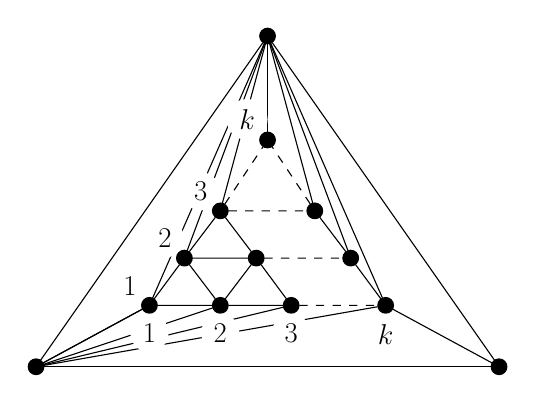
\begin{tikzpicture}[scale=1.2]
  \node (t1) at (0cm, 3.5cm) {};
  \node (t2) at (2.45cm, 0cm) {};
  \node (t3) at (-2.45cm, 0cm) {};

  \node (k1) [label=below:$1$, label=above left:$1$] at (-1.25cm, 0.65cm) {};
  \node (k2) [label=below:$2$]  at (-0.5cm, 0.65cm) {};
  \node (k3) [label=below:$3$]  at (0.25cm, 0.65cm) {};
  \node (kn) [label=below:$k$]  at (1.25cm, 0.65cm) {};

  \node (l1) [label=above left:$2$]  at (-0.88cm, 1.15cm) {};
  \node (l2) at (-0.12cm, 1.15cm) {};
  \node (ln) at (0.88cm, 1.15cm) {};

  \node (j1) [label=above left:$3$] at (-0.5cm, 1.65cm) {};
  \node (jn) at (0.5cm, 1.65cm) {};

  \node (p) [label=above left:$k$]  at (0cm, 2.4cm) {};

  \begin{pgfonlayer}{bg}
	  \draw (t1) edge (t2); \draw (t3) edge (t2); \draw (t1) edge (t3);
	  \draw (k1) edge (k2); \draw (k3) edge (k2);
	  \draw (k3) edge (kn) [dashed];

	  \draw (l1) edge (l2);
	  \draw (l2) edge (ln) [dashed];

	  \draw (j1) edge (jn) [dashed];

	  \draw (j1) edge (p) [dashed];
	  \draw (jn) edge (p) [dashed];

	  \draw (t1) edge (k1); \draw (t1) edge (kn);
	  \draw (t1) edge (l1); \draw (t1) edge (ln);
	  \draw (t1) edge (p);
	  \draw (t2) edge (kn); \draw (t3) edge (k1);

	  \draw (k1) edge (l1); \draw (k2) edge (l1);
	  \draw (k2) edge (l2); \draw (k3) edge (l2);
	  \draw (kn) edge (ln);

	  \draw (l1) edge (j1); \draw (l2) edge (j1);
	  \draw (jn) edge (ln);

	  \draw (j1) edge (t1); \draw (jn) edge (t1);

	  \draw (t3) edge (k1); \draw (t3) edge (k2);
	  \draw (t3) edge (k3); \draw (t3) edge (kn);
  \end{pgfonlayer}

\end{tikzpicture}

\caption{The collection of graphs $\{G_k\}_{k\in\mathbb{N}}$ on which Poh
performs poorly.}
\label{F:poh_bad_graph_collection}
\end{center}
\end{figure}

A natural way to implement Poh's algorithm is to use a breadth-first search to
to attempt to construct the shortest path of Case 1.1 and in the process locate
a chord edge of Case 1.2 if no such path is possible. Unfortunately this method
results in an algorithm that is not linear. To see this, consider the family of
graphs $\{G_k\}_{k\in\mathbb{N}}$ depicted in
Figure \ref{F:poh_bad_graph_collection}. Fix $k\in\mathbb{N}$ and note that
$n=n(G_k)=k(k+1)/2+3$. Assume
that the outer triangle is path $2$-colored such that the top vertex
assigned a color distinct from the bottom two. At iteration $i$ of Poh's
algorithm, the shortest path through the interior will be the path of length
$l=k-i+1$ directly along the base of the inner triangle. A breadth-first search
of this inner triangle will hit all $l(l+1)/2$ vertices in order to find this
path. Therefore the total number of operations performed will be
\[
    \Theta\left( \sum_{l=1}^k\frac{l(l+1)}{2} \right)=\Theta(n^{3/2}).
\]
So Poh's algorithm with breadth-first search is $\Omega(n^{3/2})$.

However, the correctness of Poh's algorithm did not rely on
locating the shortest $uw$-path, only on locating some induced $uw$-path.
Below we will see that modifying Poh's algorithm to locate induced paths will
allow us produce a linear time implementation.

The general strategy will be to walk clockwise along the colored path
$P_1=v_1,v_2,\ldots,v_l$ in the outer cycle $C$, marking those vertices
interior to $C$ that have a neighbor in $P_1$. We will then construct an
induced path $P_3=u_1,u_2,\ldots,u_d$, consisting only of marked vertices,
such that $C_1=P_1\cup P_3\cup\{u_1v_1,u_dv_l\}$ is a cycle and all marked
vertices are contained in the subgraph of $G$ bounded by $C_1$. 


\section{Path List Coloring: the Hartman-\v{S}krekovski Algorithm}

ZZZ


\begin{thebibliography}{99}

\bibitem{BoMy2004}
J.~Boyer and W.~Myrvold, On the cutting edge: simplified $O(n)$ planarity by edge
addition,
\textit{J. Graph Algorithms Appl.}
\textbf{8} (2004),
241--273.

\bibitem{BrMy1985}
I.~Broere and C.~M.~Mynhardt,
Generalized colorings of outerplanar and planar graphs,
\textit{Graph theory with applications to algorithms and computer science}
 (Kalamazoo, Mich., 1984),
pp.~151--161,
Wiley-Intersci. Publ., Wiley, New York, 1985.

\bibitem{Bro2017}
A.~Bross,
\textit{Implementing path coloring algorithms on planar graphs},
Masters Project,
University of Alaska,
2017,
available from\hfil\break
\texttt{http://github.com/permutationlock/path\_coloring\_bgl}.

\bibitem{ChHa2017prep}
G.~G.~Chappell and C.~Hartman,
Path choosability of planar graphs,
in preparation.

\bibitem{ChKr1969}
G.~Chartrand and H.~V.~Kronk,
The point-arboricity of planar graphs,
\textit{J. London. Math. Soc.}
\textbf{44} (1969),
612--616.

\bibitem{God1991}
W.~Goddard,
Acyclic colorings of planar graphs,
\textit{Discrete Math.}
\textbf{91} (1991), no. 1,
91--94.

\bibitem{Har1997}
C.~M.~Hartman,
\textit{Extremal Problems in Graph Theory},
Ph.D. Thesis,
University of Illinois,
1997.

\bibitem{Poh1990}
K.~S.~Poh,
On the linear vertex-arboricity of a planar graph,
\textit{J. Graph Theory}
\textbf{14} (1990), no. 1,
73--75.

\bibitem{Skr1999}
R.~\v{S}krekovski,
List improper colourings of planar graphs,
\textit{Combin. Probab. Comput.}
\textbf{8} (1999), no. 3,
293--299.

\bibitem{Wes2000}
D.~B.~West,
\textit{Introduction to Graph Theory, 2nd ed.},
Prentice Hall,
Upper Saddle River, NJ,
2000.

\end{thebibliography}

\end{document}

